% Header mit Deklarationen
\documentclass[
    pdftex,             % PDFTex 
    a4paper,            % A4 Papier
    oneside,            % einseitig
    liststotoc,         % Verzeichnisse einbinden in toc
    halfparskip,        % Abstand zwischen Absätzen
    chapterprefix,      % Kapitel ausschreiben
    headsepline,        % Linie nach Kopfzeile
    %footsepline,       % Linie vor Fusszeile
    pointlessnumbers,   % Nummern ohne abschließenden Punkt
    12pt                % Schriftgröße
]{scrbook}

%
% Randabstände
%
\usepackage[]{geometry}

%
% Paket Deutsch
%
\usepackage[ngerman]{babel}

%
% Pakete für UTF-8
%
\usepackage[utf8]{inputenc}
\usepackage[T1]{fontenc}

%
% Anführungszeichen
%
\usepackage[babel,german=quotes]{csquotes}

% 
% Verweise mit Autor und Jahr
%
\usepackage{natbib}
\bibliographystyle{abbrvnat}

%
% Paket für Tabelleneigenschaften
%
\usepackage{array}

%
% Paket für Tabellen
%
\usepackage{booktabs}

%
% Paket für Grafiken
%
\usepackage{graphicx}

%
% Spezielle Schrift setzen
%
\setkomafont{sectioning}{\normalfont\bfseries}
\setkomafont{captionlabel}{\normalfont\bfseries} 
\setkomafont{pagehead}{\normalfont\fontsize{9.5pt}{11.4pt}} % Kopfzeilenschrift
\setkomafont{descriptionlabel}{\normalfont\bfseries}

%
% Zeilenumbruch bei Bildbeschreibungen
%
\setcapindent{1em}

%
% Kopf und Fußzeilen
%
\usepackage[automark,autooneside=false]{scrlayer-scrpage}
\pagestyle{scrheadings}
\automark[section]{chapter}
\ihead{\leftmark}
\ohead{\rightmark}
\chead{}

%
% Mathematische Symbole
%
\usepackage{amsmath}
\usepackage{amssymb}

%
% Type 1 Fonts für bessere Darstellung in PDF verwenden.
%
%\usepackage{mathptmx}           % Times
\usepackage{helvet}              % Helvetica
\renewcommand{\familydefault}{\sfdefault}
\usepackage{courier}             % Courier

%
% Paket für Farben im PDF
%
\usepackage{color}

%
% Paket für Links innerhalb des PDF Dokuments
%
\definecolor{LinkColor}{rgb}{0,0,0}
\usepackage[%
	pdftitle={Titel},                        % Titel der Arbeit
	pdfauthor={Autor},                       % AutorIn
	pdfcreator={LaTeX},                      % genutzte Programme
	pdfsubject={Betreff},
	pdfkeywords={Keywords}]{hyperref}
\hypersetup{colorlinks=true, linkcolor=LinkColor, 
            citecolor=LinkColor, filecolor=LinkColor, 
            menucolor=LinkColor, pagecolor=LinkColor, urlcolor=LinkColor}                                       

%
% Paket um Listings zu formatieren
%
\usepackage[savemem]{listings}
\lstloadlanguages{TeX}


%
% Neue Umgebungen
%
\newenvironment{ListChanges}%
	{\begin{list}{$\diamondsuit$}{}}%
	{\end{list}}

%
% aller Bilder im Unterverzeichnis 'bilder' gesucht
%
\graphicspath{{bilder/}}

%
% Strukturiertiefe bis subsubsection{} möglich
%
\setcounter{secnumdepth}{3}

%
% Dargestellte Strukturiertiefe im Inhaltsverzeichnis
%
\setcounter{tocdepth}{3}

%
% Abkürzungsverzeichnis
%
\usepackage[intoc]{nomencl}
\usepackage[toc]{glossaries}
\makeglossaries
\renewcommand*\glspostdescription{\dotfill}


\begin{document}

% Titelblatt
%% Titelseite
%% Vorlage $Id: titelseite.tex 61 2012-05-03 13:58:03Z bless $

\def\usesf{}
\let\usesf\sffamily % diese Zeile auskommentieren für normalen TeX Font

\newsavebox{\Erstgutachter}
\savebox{\Erstgutachter}{\usesf xxxxxxxxxx}
\newsavebox{\Zweitgutachter}
\savebox{\Zweitgutachter}{\usesf xxxxxxxxxx}
\newsavebox{\Betreuer}
\savebox{\Betreuer}{\usesf xxxxxxxxxx}

\begin{titlepage}
\setlength{\unitlength}{1pt}
\begin{picture}(0,0)(85,770)
%\includegraphics[width=\paperwidth]{logos/KIT_Deckblatt}
\end{picture}

\thispagestyle{empty}

%\begin{titlepage}
%%\let\footnotesize\small \let\footnoterule\relax
\begin{center}
\hbox{}
\vfill
{\usesf
{\huge\bfseries Titel der Abschlussarbeit \par}
\vskip 1.8cm
{\huge Bachelorarbeit / Masterarbeit}\\
\vskip 0.5cm
zur Erlangung des akademischen Grades\\
Bachelor/Master of Science (B.Sc./M.Sc.) 
\vskip 1.5cm

{\large Universität Trier\\
FB IV - Informatikwissenschaften\\
Professur Wirtschaftsinformatik I / II\\}

\vskip 3cm
\begin{tabular}{p{3.5cm}l}
Gutachter: & \usebox{\Erstgutachter} \\
 & \usebox{\Zweitgutachter} \\
Betreuer: & \usebox{\Betreuer} \\
\end{tabular}
\vskip 3cm
Vorgelegt am xx.xx.xxxx von:\\
\vskip .5cm
Vorname Nachname\\
Anschrift\\
PLZ Stadt\\
E-Mail-Adresse\\
Matr.-Nr. 123456


}
\end{center}
\vfill
\end{titlepage}
%% Titelseite Ende


%%% Local Variables: 
%%% mode: latex
%%% TeX-master: "thesis"
%%% End: 


% Eidesstattliche Erklärung
%
% Inhaltsverzeichnis
%
\clearpage% oder \cleardoublepage bei twoside
\begingroup
  \renewcommand*{\chapterpagestyle}{empty}
  \pagestyle{empty}
  % Die eidesstattliche Erklärung mit Unterschrift
\chapter*{Erklärung der Urheberschaft}

Ich erkläre hiermit an Eides statt, dass ich die vorliegende Arbeit
ohne Hilfe Dritter und ohne Benutzung anderer als der angegebenen
Hilfsmittel angefertigt habe; die aus fremden Quellen direkt oder
indirekt übernommenen Gedanken sind als solche kenntlich gemacht. Die
Arbeit wurde bisher in gleicher oder ähnlicher Form in keiner anderen
Prüfungsbehörde vorgelegt und auch noch nicht veröffentlicht.

\vspace{4cm}

\hspace{2cm} Ort, Datum \hfill Unterschrift \hspace{2cm}

  \tableofcontents
  \clearpage
\endgroup

\setcounter{page}{1}
% Römische Nummerierung für Sonderseiten, wie Verzeichnisse und Anhang
\pagenumbering{Roman}

% Verzeichnisse
% Kopfzeile links Kapitel, rechts leer
\ihead{\leftmark}
\ohead{}

%
% Abbildungsverzeichnis
%
\listoffigures

%
% Abkürzungsverzeichnis
%
% 
% Liste von Abkürzungen, die im gesamten Dokument mit \gls{-label-} referenziert werden können.
% \newacronym{<label>}{<abbrv>}{<full>}
%
\newacronym{etc}{etc.}{et cetera}
\newacronym{usw}{usw.}{und so weiter}

\printglossary[title=Abkürzungsverzeichnis]
%\printglossaries

%
% Tabellenverzeichnis
%
\listoftables


% Merke mir die römische Seitenzahl in 'roemisch' und setzte Nummerierung 
% auf arabisch für die eigentlichen Kapitel
\newpage
\newcounter{roemisch}
\setcounter{roemisch}{\value{page}}
\pagenumbering{arabic}

% Die einzelnen Kapitel
% Kopfzeile: links Kapitel, rechts Sektion
%\ihead{\leftmark}
%\ohead{\rightmark}
\ihead{\parbox[t][2\baselineskip][t]{\dimexpr\linewidth-2em\relax}{\leftmark}}
\ohead{\parbox[t][2\baselineskip][t]{20em}{\raggedleft\rightmark}}
\chapter{Einleitung}

Als Textgenerierung (auch natürlichsprachliche Generierung; englisch Natural Language Generation, NLG) bezeichnet man die automatische Produktion von natürlicher Sprache durch eine Maschine. Die Generierung von Texten ist als Teilbereich der Computerlinguistik eine besondere Form der künstlichen Intelligenz. 
Die maschinelle Übersetzung wird in der Regel von einem professionellen Übersetzer durchgeführt, der die Übersetzung in die Zielsprache übersetzt, bevor er die entsprechende Übersetzung anfertigt, um die Qualität des Ausgangstextes zu gewährleisten und die Genauigkeit der Übersetzung zu garantieren, die in den meisten Fällen durch die maschinellen Übersetzungen erreicht wird. ...
Diese Maschine ist in der Lage, eine komplette Reihe von Sprachen zu erzeugen, die in den folgenden Kapiteln beschrieben werden.

\chapter{Zweites Kapitel}

\section{Fließtext mit Verweis und Abbildung}

%
%   Verweis im Text bei Nennung des Autors (citet) oder in Klammern (citep) 
%
Dies ist der Grund, so \citet{jurafsky2009}, warum sich die meisten Übersetzungsbüros 
für diese Art der Übersetzung entscheiden.
Der Übersetzungsservice (Abbildung~\ref{fig:bildlabel1}) wird von einem Team von 
Fachleuten \citep[S. 3]{mikolov2013} mit langjähriger Erfahrung im Bereich der 
Übersetzungswissenschaft und des Dolmetschens durchgeführt.

%
%   Grafik einfügen
%
\begin{figure}[htbp]
\centering
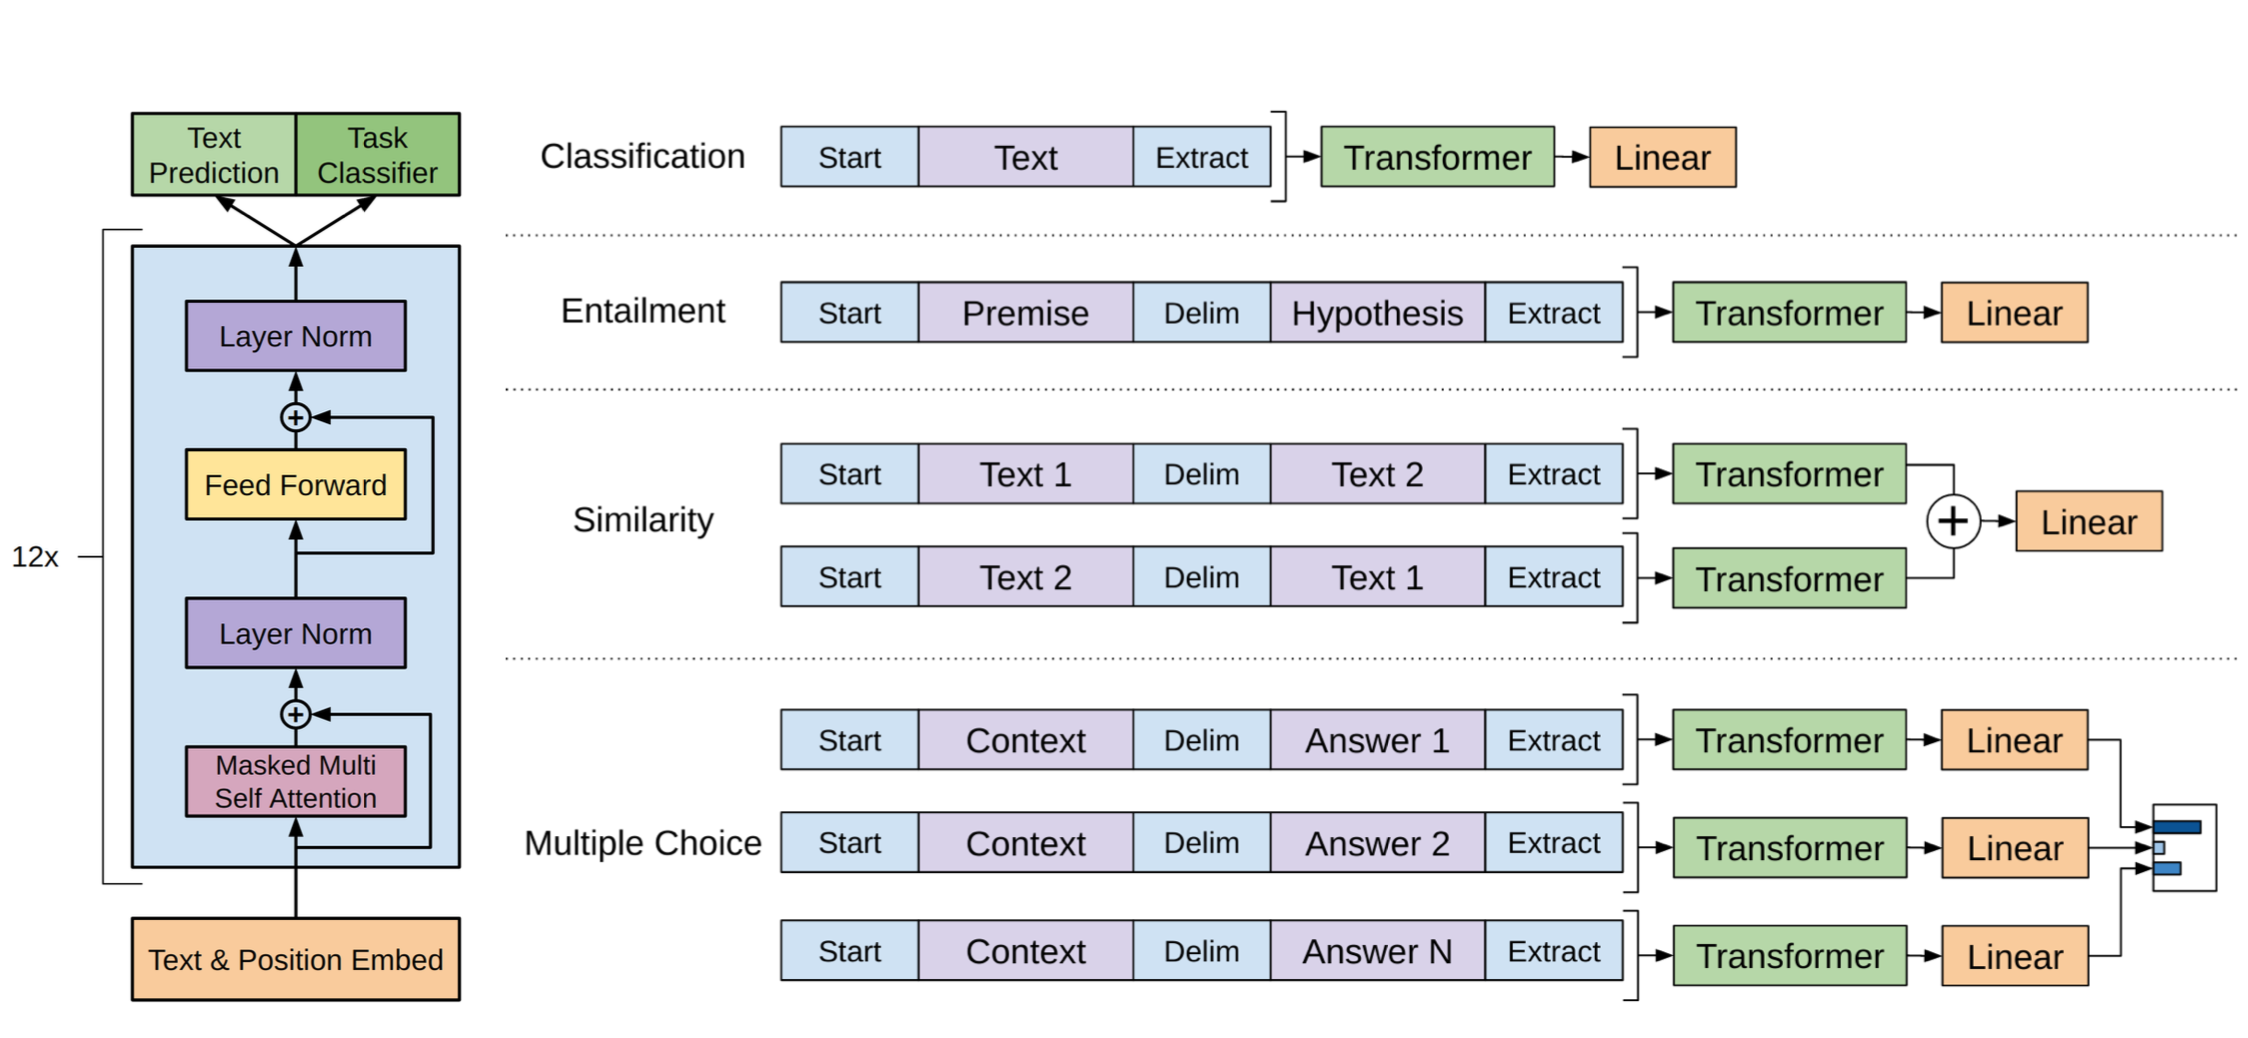
\includegraphics[width=0.5\textwidth]{gpt-model-open-ai-2018}
\caption{GPT-Modell} 
\label{fig:bildlabel1}
\end{figure}

Das Internet ist ein sehr komplexes System, aber es ist sehr leicht zu verstehen, warum es so viele Möglichkeiten gibt, dieses System zu nutzen, obwohl es viele verschiedene Möglichkeiten hat, diesen Prozess zu automatisieren, nämlich die Übertragung von Daten zwischen Computern und Servern, sowie die Verteilung von Nachrichten zwischen den Computern, also zwischen dem PC und dem Server (das heißt, er kann sich auf eine bestimmte Art und Weise mit diesen Computern verbinden und diese Daten an andere Computer weiterleiten, anstatt sie direkt auf den PC zu übertragen).

%
%   Grafik einfügen
%
\begin{figure}[htbp]
\centering
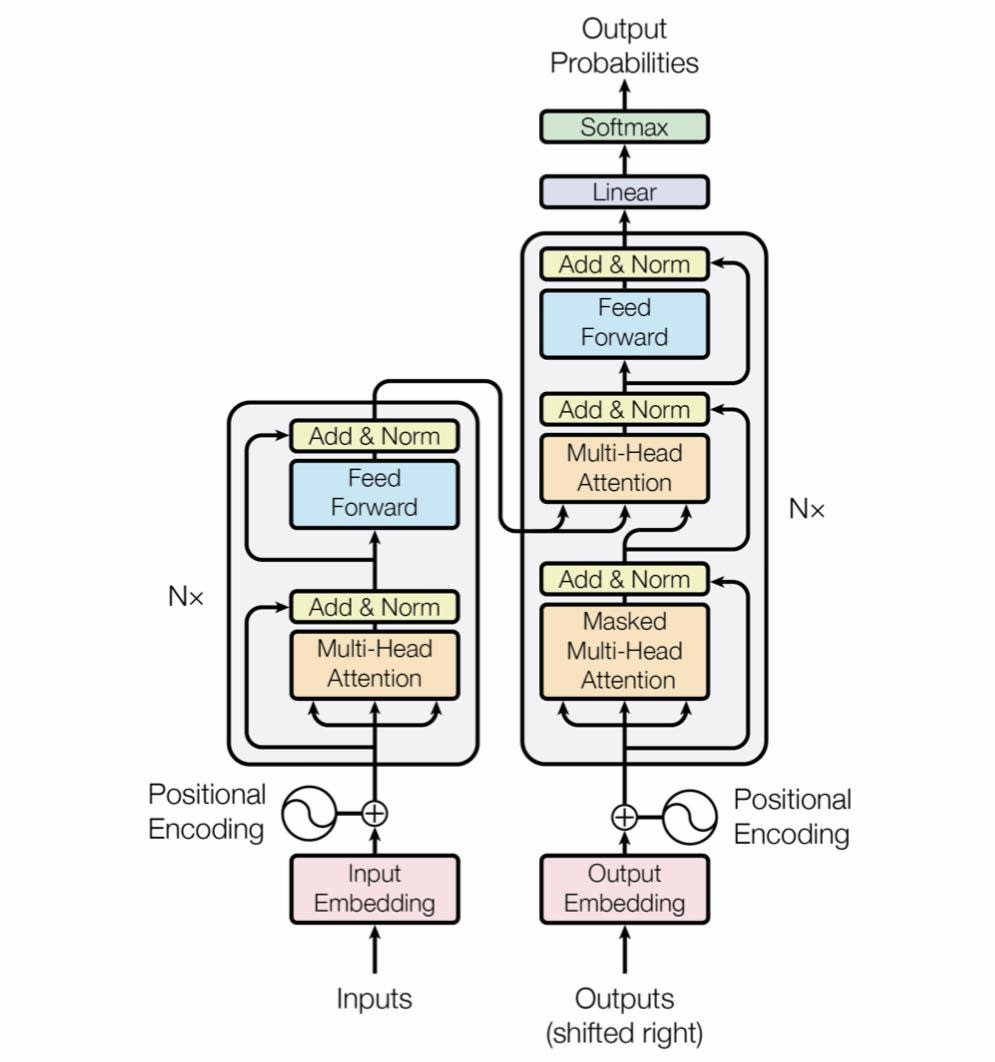
\includegraphics[width=0.8\textwidth]{gpt2}
\caption{Der Titel der Abbildung} 
\label{fig:bildlabel2}
\end{figure}

Das Übersetzungsbüro (Abbildung~\ref{fig:bildlabel1}) bietet eine breite Palette von Übersetzungsdienstleistungen an, angefangen bei der Auswahl der Sprachen für die jeweilige Sprache, bis hin zur Erstellung von Übersetzungen für jede Sprache und für jedes Format, das für den jeweiligen Kunden am besten geeignet ist (z. B. Chinesisch, Koreanisch, Arabisch, Thai, Vietnam, usw.).

\section{Abkürzung und Anführungszeichen im Text}

%
% Beispiel Abkürzung
%
Eine Abkürzung ist z.B. \gls{etc}, die im Abkürzungsverzeichnis erklärt wird. Beim erneuten Vorkommen der Abkürzung \gls{etc} wird nur noch diese gedruckt.

%
% Beispiel Anführungszeichen
%
Anführungszeichen kann man entweder \enquote{so} erstellen oder mit UTF8-encodierter Quelldatei auch „so“.
Der Computer ist ein \enquote{Computer}, in dem sich der \enquote{Benutzer} befindet und der sich mit ihm in \enquote{Verbindung} setzt, so dass er von ihm gesteuert werden kann, ohne dass ihm der Zugang zum Computer verwehrt wird (wenn er das nicht tut, ist er gezwungen, ihn auszuschalten, da er die Kontrolle über das Computersystem hat), oder er kann sich selbst nicht an einen Computer anschließen, indem er sich an eine beliebige andere Maschine anschließt (es ist nicht möglich, ein Programm zu installieren, welches die ganze Maschine ausführt, selbst wenn es nicht funktioniert);

\section{Beispiel Fußnote}

%
%   Beispiel Fußnote mit Referenz
%   Die Referenz A muss in bib.bib enthalten sein
%
Dieses Programm\footnote{vgl. \cite{jurafsky2009}}
ist sehr einfach zu bedienen, da es die Möglichkeit\footnote{Dies ist eine Fußnote ohne Referenz}
bietet, eine Reihe von Funktionen zu implementieren, von denen die meisten für die Programmierung von Programmiersprachen geeignet sind.

\section{Beispiel Tabelle}

Der Text wird dann in ein anderes Format (siehe in Tabelle~\ref{tab:tabellenlabel1}) 
konvertiert, das dann als die Originaldatei bezeichnet wird, wenn der Text in einer anderen Form vorliegt, als das Original, wobei die ursprüngliche Übersetzung unverändert bleibt, bis die originale Übersetzung erneut verwendet wird.

%
%   Beispiel Tabelle
%
\begin{table}[htbp]
\centering
\begin{tabular}{l|l|l|l}
SpalteA & SpalteB & SpalteC & SpalteD \\
\midrule
A1 & B1 & C1 & D1 \\
A2 & B2 & C2 & D2 \\
A3 & B3 & C3 & D3
\end{tabular}
\caption{Beispiel einer Tabelle}
\label{tab:tabellenlabel1}
\end{table}

Sie ist in der Lage, in einem einzigen Arbeitsschritt die Sprache zu programmieren und zu übersetzen, ohne dass es sich dabei um eine maschinelle Übersetzung handelt, die sich auf die Übersetzung der Originalsprache bezieht, wie sie von den meisten anderen Übersetzungsdienstleistern verwendet wird (z.B. von Google, Yahoo, etc.).
Die automatische Übersetzung von Quelltext in die Zielsprache ist eine der am häufigsten verwendeten Formen der maschinellen Übersetzung, wenn es um die Übertragung von Text in eine andere Sprache geht, d.h. eine Übersetzung in mehrere Sprachen, z. B. Englisch, Französisch, Deutsch, Italienisch, Spanisch, Portugiesisch, Russisch, Niederländisch, Polnisch, Schwedisch, Dänisch oder Norwegisch (oder umgekehrt).

\chapter{Drittes Kapitel}

\section{Aufzählungen und Unter-unterkapitel}

\subsection{einfache Liste}

Diese Methode wird in der Naturwissenschaft als "automatische Übersetzung" bezeichnet, bei der die Übersetzung in eine andere Sprache als in einer anderen Sprache (z.B. in Japanisch, Koreanisch, Deutsch, Englisch, Französisch, Italienisch, Spanisch, Polnisch, Portugiesisch, Russisch, Schwedisch usw.) erfolgen muss, um die gewünschte Zielsprache zu erhalten (siehe oben).

\begin{itemize}
 \item erstes Element
 \item zweites Element
 \item Element Nummer drei
\end{itemize}

Die meisten Maschinen zeichnen sich durch ihre Einfachheit und Einfachheit aus, aber die meisten dieser Maschinen sind nicht für den professionellen Gebrauch bestimmt.

\subsection{nummerierte Liste}

Diese Maschine ist die einzige Maschine, die es erlaubt, jede beliebige Anzahl von Wörtern in einer Sprache zu schreiben, unabhängig davon, ob es sich dabei um eine oder mehrere Wörter handelt, oder ob sie sich um ein oder zwei Wörter oder um zwei oder mehr Wörter handeln muss, um einen Text zu erzeugen.

\begin{enumerate}
 \item erster Punkt
 \item weiterer Punkt
 \item letzter Punkt
\end{enumerate}

Die maschinelle Übersetzung wird durch die Maschine selbst durchgeführt, d.h. durch einen Übersetzer, der das Ergebnis der maschinellen Übersetzung mit Hilfe der Software selbst auswählt, oder durch den Übersetzer in einem anderen Land als dem, in dem er sich aufhält, wo er arbeitet und wo es ihm möglich ist, seine Muttersprache zu sprechen (im Gegensatz zu anderen Sprachen, die in anderen Ländern als Muttersprache gesprochen werden).

\section{Formeln}

Die Maschine besteht aus der Exponentialfunktion 
$e^x = \lim_{n \to \infty} \left( 1+ \frac{x}{n} \right)^n$ 
und dem Codegenerator, der mit dem Computer verbunden 
ist und der Software, mit der der Code generiert werden kann, 
um die Software zu programmieren und zu schreiben, und die 
Maschine kann in verschiedenen Sprachen verwendet werden.

\begin{align}
\label{bayes}
    P(A \mid B) = \frac{P(B \mid A) \, P(A)}{P(B)}
\end{align}

Im Gegensatz zu den meisten anderen Programmen können wir keine Programmiersprache benutzen, weil wir die Sprache nicht beherrschen, sondern nur lernen, sie zu verstehen und sie in andere Sprachen zu übersetzen, damit wir sie verstehen können und mit ihnen arbeiten können (d. h. mit ihr arbeiten)


% Setze Numerierung wieder auf römisch zurück und setzte von oben fort
% Wert ist demnach der von 'roemisch'
\newpage
\pagenumbering{Roman}
\setcounter{page}{\value{roemisch}}

% Literaturverzeichnis
\bibliography{literatur/bib}

% Anhänge, falls vorhanden
\appendix
% Anhänge
\chapter{Quellcode}

\begin{lstlisting}[language=Python]
import numpy as np
    
def incmatrix(genl1,genl2):
    m = len(genl1)
    n = len(genl2)
    M = None #to become the incidence matrix
    VT = np.zeros((n*m,1), int)  #dummy variable
    
    #compute the bitwise xor matrix
    M1 = bitxormatrix(genl1)
    M2 = np.triu(bitxormatrix(genl2),1) 

    for i in range(m-1):
        for j in range(i+1, m):
            [r,c] = np.where(M2 == M1[i,j])
            for k in range(len(r)):
                VT[(i)*n + r[k]] = 1;
                VT[(i)*n + c[k]] = 1;
                VT[(j)*n + r[k]] = 1;
                VT[(j)*n + c[k]] = 1;
                
                if M is None:
                    M = np.copy(VT)
                else:
                    M = np.concatenate((M, VT), 1)
                
                VT = np.zeros((n*m,1), int)
    
    return M
\end{lstlisting}


\end{document}
